\documentclass[xetex,mathserif,serif]{beamer}

\title[Query Visualization] % (optional, only for long titles)
{Visualizing Physical Query Execution in a Relational Distributed Big Data Management System}
\subtitle{}
\author[Chu, moritz] % (optional, for multiple authors)
{Shumo Chu, Dominik Moritz}

\begin{document}

\begin{frame}
\titlepage
\end{frame}

\begin{frame}
\frametitle{The Myria System}
\begin{enumerate}
	\item Big Data management system developed in db group
	\item Pipelined, parallel, distributed dataflow evaluation system
	\item \textbf{Fragments}: trees of operators that are each executed on one thread in each worker
	\item Fragment leaves and roots are typically I/O operators
\end{enumerate}
\end{frame}

\begin{frame}
\frametitle{Myria Architecture}
\begin{figure}
 \begin{center}
     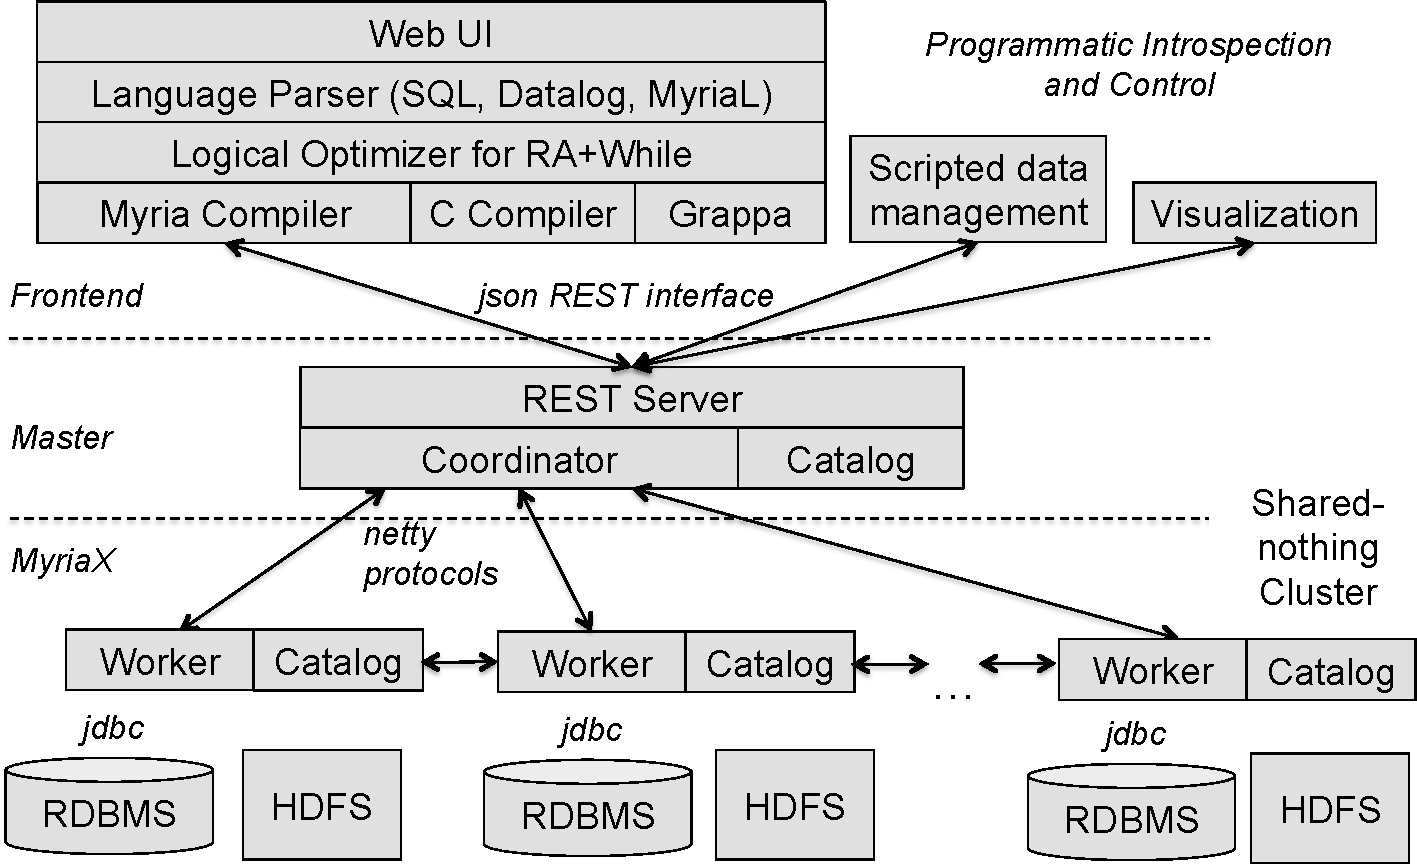
\includegraphics[width=0.9\textwidth]{arch}
   \end{center}
  \caption{Myria System Architecture.}
  \label{fig:myria_arc}
\end{figure}
\end{frame}

\begin{frame}
\frametitle{System architecture}
Image that shows how we fetch logs and where app engine is.
\end{frame}

\end{document}